\section{Install packages}
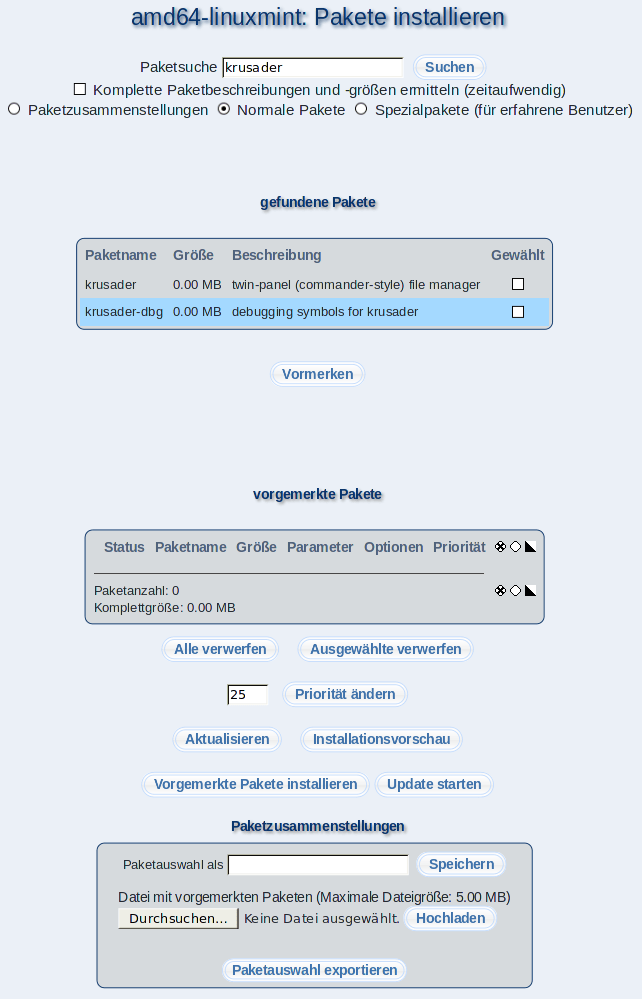
\includegraphics[scale=0.4]{/mdk/doc/manual/screenshots/en/install_packages.png} \\
\subsection{Hint}
m23 differentiates between three kinds of packages:\\
\begin{itemize}
\item \textbf{Package selection:} Are a selection of different software packages. You can make selections like \textit{"office selection"} or \textit{"graphic workstation selection"}. So you don't have to select each single software package but you can use the package selection.\\
\item \textbf{Normal packages:} Are the normal software packages. They are mostly single applications.\\
\item \textbf{Special packages (for skilled users only):} Are packages for special tasks like formatting, setting of network options etc. Special packages should only be used by skilful users.\\
\end{itemize}
\subsection{Installation of packages:}
\begin{enumerate}
\item  Select \textit{"Package selection"}, \textit{"Normal packages"} or \textit{"Special packages (for skilled users only)"}.\\
\item  Enter your search key at \textit{"Package search"}. If you leave the field blank all packages matching the package criteria are displayed. Please note that this doesn't work if you select \textit{"Normal packages"} because of the huge amount of normal packages.\\
\item  At \textit{"Found packages"} you can see all packages matching your search criteria.\\
\item  Check the checkbox beside all the packages you want to install.\\
\item  Preselect your chosen packages by clicking on \textit{"Preselect"}.\\
\item  Repeat step 1-5 if required.\\
\end{enumerate}
Complete the installation by clicking on \textit{"Install preselected packages"}.\\
Now you have preselected packages for installation. A green check mark shows that the package will be installed on the client and a red cross that the package will be removed. You can remove packages from the installation list by checking the packages and clicking on \textit{"Discard selected"} or all packages by clicking on \textit{"Discard all"}.\\
Install the packages with a clic on \textit{"Install selected packages"}.\\
\subsection{Installation preview}
Before you start the real installation, you can test what will happen during installation. You can check, which additional packages will be installed or if there will be problems. Simply click on the \textit{"Installation preview"} button. After some time you will see the previewed installation protocol.\\
An installation preview works for a single client only.\\
\subsection{Hint for package selections}
If you select a package selection, you can choose the action for the packages. You have the possibility to install or deinstall the packages on or from the client. Or you can keep the stored action. This makes it possible to store installation and deinstallation jobs in the same package selection. Simply select the desired action from the selection list.\\
\subsection{Hint}
If you want to save your package selection, enter a name for the selection at \textit{"Save package selection as"} and click the \textit{"Save"} button. Afterwards, you can use your selection as a \textit{"Package selection"}.\\
